\section{Решение дифференциальных уравнений}

\AddProb
Экспериментально установлено, что при движении пули массы $m$ в деревянной доске сила сопротивления пропорциональна скорости пули по закону $\vec{F} = - \alpha \vec{v}$. Какой путь пройдет пуля в доске до остановки, если начальная скорость пули $v_0$?

\AddProb При движении тел в воздухе на них действует сила сопротивления пропорциональная квадрату скорости $F = - \alpha v^2$. По какому закону изменяются скорость и пройденный путь телом массы $m$?

%Черепанов
\AddProb Стальной шарик падает с высоты $h$ с нулевой начальной скоростью на стальную плиту. Сопротивление воздуха пропорционально квадрату скорости шарика, коэффициент пропорциональности $k$. Удар о плиту абсолютно упругий. На какую высоту $\Delta h$ шарик не долетит до начального положения при первом отскоке?

\begin{wrapfigure}{r}{5cm}
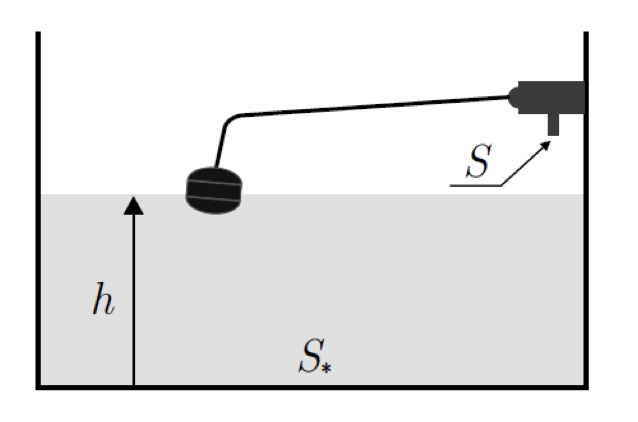
\includegraphics[scale=0.5]{ToileteTank.png}
\end{wrapfigure}

\AddProb Бачок имеет форму параллелепипеда с площадью основания $S^*$. При его наполнении водой поднимается поплавок, который постепенно закрывает кран подачи воды. Для простоты будем считать, что с увеличением уровня воды $h$ в бачке площадь отверстия крана уменьшается по линейному закону $S = S_0 (1 - h/h_{max})$. Скорость подачи воды постоянна и равна $v$. За какое время бачок полностью наполнится водой?

\AddProb В баке с площадью основания $S$ находится вода, уровень которой расположен на высоте $h_0$. Вблизи дна бака имеется небольшое отверстие площадью $s$. Как изменяется со временем уровень воды баке при истечении из отверстия?

\begin{wrapfigure}{r}{5cm}
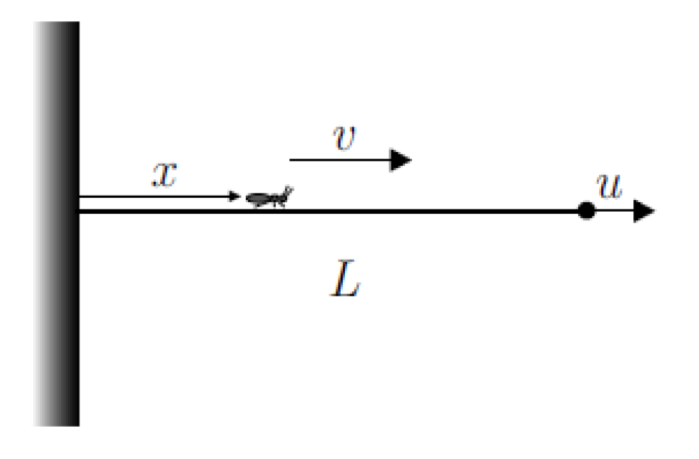
\includegraphics[scale=0.4]{AntAndTow.png}
\end{wrapfigure}
\AddProb По длинному хорошо растяжимому жгуту, один конец которого прикреплен к стене, а другой оттягивается с постоянной скоростью $u$, ползет муравей. Скорость муравья относительно жгута постоянна и равна $v$ и направлена в сторону движущегося конца жгута. Доберется ли муравей до конца жгута? За какое время? Начальная длина жгута $L_0$, муравей стартует от неподвижного конца.

\begin{wrapfigure}{r}{5cm}
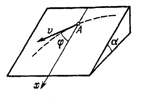
\includegraphics[scale=0.8]{WasherOnSurface.png}
\end{wrapfigure}
%Иродов
\AddProb Небольшую шайбу $A$ положили на наклонную плоскость, составляющую угол $\alpha$ с горизонтом и сообщили начальную скорость $v_0$. Найти зависимость скорости шайбы от угла $\varphi$, если коэффициент трения $k = \tan \alpha$ и в начальный момент $\varphi_0 = \pi/2$.

%Черепанов
\AddProb Наклонная плоскость имеет угол $\alpha$ с горизонтом. Тело, лежащее на наклонной плоскости, толкнули в горизонтальном направлении с начальной скоростью $v_0$. Коэффициент трения тела о плоскость равен $\mu = k \tan \alpha (k > 1)$. Через какое время тело остановится и какой путь пройдет до остановки?

%Туймадаа
\AddProb С вертикальной скалы высотой $H$ брошен горизонтально со скоростью $v_0$ камень массой $m$. Спустя некоторое время он стал двигаться с постоянной скоростью. Считая, что сила сопротивления воздуха пропорциональна скорости, найти расстояние по горизонтали $L$, на которое камень удалится от скалы в момент падения, и время движения $t$.

%16 Черепанов
\AddProb (2007) Бусинка находится в наинизшей точке вертикально расположенной неподвижной шероховатой окружности радиуса $R$. Какую минимальную скорость надо сообщить бусинке, чтобы она достигла горизонтального диаметра окружности? Коэффициент трения равен $\mu$.

% Черепанов
\AddProb (2008) Сферическая капля воды движется в однородном поле тяжести в среде, в которой за счет конденсации происходит увеличение массы капли, пропорциональное ее поверхности. Найти скорость капли в зависимости от времени, если в начальный момент времени капля была неподвижна, ее масса равнялась $m_0$. Плотность воды $\rho$.

% Жухарев
\AddProb (2008) В данной плоскости движутся две точки: точка 1 движется по прямой с постоянной скоростью $v_1$, а точка 2 – с постоянной по модулю скоростью $v_2$, направленной все время на точку 1. Найти траекторию точки 2 и координату места встречи 1 и 2. Считать, что в начальный момент времени расстояние между точками $y_0$ и $\vec{v_2} \bot \vec{v_1}$.


%\begin{wrapfigure}{r}{5cm}
%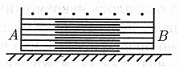
\includegraphics{0402DynamicsPaper.jpg}
%\end{wrapfigure}


\section{Дополнительные задачи}
1. Дифуравнения в механике (Иродов, МФТИ, Morin)
2. Распределенная масса, силы, канат, цепочка - добавить в основной текст 
3. Вращательное движение (моменты инерции, сохранение момента импульса)
4. Колебания (старые листы)
5. Электростатика (сферы, потенциалы, конденсаторы)
6. ЭМ индукция, сила Ампера
8. Переменный ток
9. %TODO Добавить задачи олимпиад 2015-2018 в методичку по темам  
